\documentclass{article}

\usepackage{arxiv}

\usepackage[utf8]{inputenc} % allow utf-8 input
\usepackage[T1]{fontenc}    % use 8-bit T1 fonts
\usepackage{hyperref}       % hyperlinks
\usepackage{url}            % simple URL typesetting
\usepackage{booktabs}       % professional-quality tables
\usepackage{amsfonts}       % blackboard math symbols
\usepackage{nicefrac}       % compact symbols for 1/2, etc.
\usepackage{microtype}      % microtypography
\usepackage{lipsum}
\usepackage[normalem]{ulem}
\usepackage{mathrsfs}
\usepackage{epsfig, graphicx}
\usepackage{latexsym,amsfonts,amsbsy,amssymb}
\usepackage{amsmath}
\usepackage{color}
\usepackage{mathtools}
\usepackage{float}
\usepackage{cite}
%\usepackage{algorithm,algpseudocode}
\usepackage{algorithm2e}
\usepackage{amsmath}
\usepackage{amsfonts}
\usepackage{amssymb}
\usepackage{comment}
\usepackage{caption}  % for side by side figures

\newcommand{\xb}{\mathbf{x}}
\newcommand{\sbb}{\mathbf{s}}
\newcommand{\gb}{\mathbf{g}}
\newcommand{\Hb}{\mathbf{H}}

\newcommand{\R}{\mathbb{R}}
\newcommand{\dd}{\delta}
\newcommand{\zero}{\mathbf{0}}
\newcommand{\trho}{\tilde\rho}
\newcommand{\ared}{\mathrm{ared}}
\newcommand{\pred}{\mathrm{pred}}
\newcommand{\ered}{\mathrm{ered}}
\newcommand{\gammainc}{\gamma_{\mathrm{inc}}}
\newcommand{\gammadec}{\gamma_{\mathrm{dec}}}
\newcommand{\true}{\mathrm{TRUE}}
\newcommand{\false}{\mathrm{FALSE}}

\newcommand{\algref}[1]{{\rm Algorithm~\ref{alg:#1}}}
\newcommand{\figref}[1]{{\rm Figure~\ref{fig:#1}}}

\newcommand{\mmnote}[1]{\textsf{{\color{red}{ MM:}   #1}}}
\newcommand{\phnote}[1]{\textsf{{\color{cyan}{ PH:}   #1}}}
\newcommand{\jhnote}[1]{\textsf{{\color{blue}{ JH:}   #1}}}

\usepackage{listings}
\lstset{language=C,
  basicstyle=\ttfamily,
  keywordstyle=\color{blue!80!black},
  commentstyle=\color{green!60!black}
}

\graphicspath{{images/}}

\title{Trust Region Optimization at Mixed Precision}

\author{
  Anonymous Alpaca \\
  Argonne National Laboratory \\
  \texttt{alpaca@anl.gov}
}

\begin{document}
\maketitle

\begin{abstract}
We present a method to perform trust region based optimization for nonlinear unconstrained problems. The method selectively uses function and gradient evaluations at different floating point precisions to reduce the overall power consumption and time to solution.
\end{abstract}


% keywords can be removed
\keywords{Optimization \and Trust Region Methods \and Mixed Precision}

\section{Introduction}
\label{sec:intro}
Optimization methods are used in many applications, including engineering, science, and machine learning. The memory footprint and run time of optimization methods has been studied extensively and determines the problem sizes that can be run on existing hardware. Similarly, the power consumption of optimization methods determines their cost and carbon footprint, which is recently becoming a growing concern~\cite{hao2019training}. Previous work has found significant differences in the overall power consumption for double and single precision computations~\cite{molka2010characterizing}. TODO: Plenty of work on power consumption overall, few specific to scientific computing (e.g.~\cite{kestor2013quantifying}), but there is not much about concrete factors between single/double.

Also TODO: Should we have an acronym, and if so, which one? Let's collect ideas here. Filler words like "for", "at", "with" can be added as needed.
\begin{itemize}
    \item \sout{TROMP - Trust Region Optimization Mixed Precision}
    \item \sout{TROUT - Trust Region Optimization UnconsTrained Problems}
    \item TRUMP - Trust Region method Using Mixed Precision
    \item \sout{UMMPA - Unconstrained Minimization Mixed Precision Arithmetic}
    \item \sout{TRUMPET - TRUst region Mixed Precision arithmETic}
\end{itemize}
\mmnote{Come on guys. Was this even a question?} 

\section{Background}
\label{sec:related}
Related work~\cite{strzodka2006mixed}.

Probably the most relevant related paper, need to be clear how we improve over their work~\cite{gratton2018note}.

\section{Method}
\label{sec:method}

\textbf{We can integrate text into earlier sections as required. I'm just trying to create consistent notation and a self-contained algorithm description for now.}

We consider the unconstrained minimization of a differentiable function $f:\R^n\to\R$,
\begin{equation}
\label{eq:unc}
 \displaystyle\min_{\xb\in\R^n} f(\xb).
\end{equation}
We suppose that we have access to a hierarchy of arithmetic precisions for the evaluation of both $f(\xb)$ and $\nabla f(\xb)$,
but the direct evaluation of $f(\xb),\nabla f(\xb)$ is unavailable. 
We formalize this slightly by supposing we are given oracles that compute $f^p(\xb), \nabla f^p(\xb)$ for $p\in\{1,\dots,P\}$. 
At a majority of input $\xb$, the relation
\begin{equation*}
 |f^p(\xb)-f(\xb)| > |f^{p+1}(\xb)-f(\xb)|, \quad \|\nabla f^p(\xb) - \nabla f(\xb)\| > \|\nabla f^{p+1}(\xb)-\nabla f(\xb)\|
\end{equation*}
 is expected to hold for $p=1,\dots,P-1$.
 For a tangible example, if intermediate computations involved in the computation of $f(\xb)$ can be done in half, single, or double precision,
 then we can denote $f^1(\xb)$ as the oracle using only half precision computations, $f^2(\xb)$ as the oracle using only single precision,
 and $f^3(\xb)$ as the oracle using only double precision. 

 We now propose a trust-region method for the solution of \eqref{eq:unc}.
 Trust-region methods are iterative methods for optimization, and we will denote the iteration counter by $k$. 
 Given an \emph{incumbent point} $\xb_k$ in the $k$th iteration, a standard trust-region method builds some smooth model 
 $m_k:  \R^n  \to \R$
 of the function $\sbb \mapsto f(\xb_k+\sbb)$.
 The model $m_k$ is intended to be ``good'' in a sense to be formalized later on the \emph{trust-region}
 $\{\sbb\in\R^n: \|\sbb\|\leq\dd_k\}$ for $\dd_k>0$, the \emph{trust-region radius}. 
 A \emph{trial step} $\sbb_k$ is then computed via a(n approximate) solution to the \emph{trust-region subproblem}
 \begin{equation}
  \label{eq:trsp}
  \displaystyle\min_{\sbb\in\R^n} m_k(\sbb): \|\sbb\|\leq\dd_k.
 \end{equation}
We formalize in the appendix \mmnote{TODO} the condition imposed on the quality of the approximate solution $\sbb_k$ to \eqref{eq:trsp},
but remark now to the reader familiar with trust-region methods that it just a standard Cauchy decrease condition. 
Having computed $\sbb_k$, the standard trust-region method then compares the true decrease in the function obtained at the trial point $\xb_k+\sbb_k$
compared to the incumbent point $\xb_k$, 
$f(\xb_k)-f(\xb+\sbb_k)$ with the decrease predicted by the model,
$m_k(\zero)-m_k(\sbb_k)$. 
In particular, one computes the quantity
\begin{equation}
 \label{eq:rho_true}
 \rho_k=\displaystyle\frac{f(\xb_k)-f(\xb_k+\sbb_k)}{m_k(\zero)-m_k(\sbb_k)}.
\end{equation}
If $\rho_k$ is sufficiently positive ($\rho_k>\eta_1$ for fixed $\eta_1>0$), then the algorithm accepts $\xb_k+\sbb_k$ as the incumbent point $\xb_{k+1}$ and may possibly
increase the trust-region radius $\dd_{k}<\dd_{k+1}$ (if $\rho_k>\eta_2$ for fixed $\eta_2\geq\eta_1$).
This scenario is called a \emph{successful iteration}. 
On the other hand, if $\rho_k$ is not sufficiently positive (or is negative), then the incumbent point $\xb_{k+1}=\xb_k$ 
and $\dd_{k} > \dd_{k+1}$.

From this basic algorithm description, we can identify two additional difficulties presented in the multiple precision setting. 
First, it is presently unclear how to compute $\rho_k$ in \eqref{eq:rho_true}, since we assumed that we have no access to an oracle that directly computes $f(\cdot)$.
Second, because models $m_k$ are typically constructed from function and gradient information provided by $f(\cdot),\nabla f(\cdot)$,
we must identify appropriate conditions on $m_k$.

For the first of these issues, we make a practical assumption that \textbf{the highest level of precision available to us should be treated as if it were real precision.}
Although this is a theoretically poor assumption, virtually all computational optimization makes this assumption implicitly; optimization methods are typically analyzed
as if computation can be done in real precision, but are only ever implemented at some level of arithmetic precision (typically double). 
Thus, in the notation we have developed, the optimization problem we actually aim to solve is not \eqref{eq:unc}, but 
\begin{equation}
\label{eq:unc_real}
 \displaystyle\min_{\xb\in\R^n} f^P(\xb)
\end{equation}
so that the $\rho$-test in \eqref{eq:rho_true} is replaced with
\begin{equation}
 \label{eq:rho}
 \rho_k=\displaystyle\frac{f^P(\xb_k)-f^P(\xb_k+\sbb_k)}{m_k(\zero)-m_k(\sbb_k)}=\displaystyle\frac{\ared_k}{\pred_k}.
\end{equation}
We introduced $\ared$ to denote ``actual reduction'' and $\pred$ to denote ``predicted reduction''. 
However, computing \eqref{eq:rho} still entails two evaluations of the highest-precision oracle $f^P(\cdot)$, and the intention of using mixed precision
was to avoid exactly this behavior. 
Our algorithm avoids the cost of full-precision evaluations 
by dynamically adjusting the precision level $p_k\in\{1,\dots,P\}$ between iterations so that in the $k$th iteration, $\rho_k$ is approximated by
\begin{equation}
 \label{eq:rho_observed}
 \trho_k=\displaystyle\frac{f^{p_k}(\xb_k)-f^{p_k}(\xb_k+\sbb_k)}{m_k(\zero)-m_k(\sbb_k)}=\displaystyle\frac{\ered_k}{\pred_k},
\end{equation}
introducing $\ered$ to denote ``estimated reduction''. 
To update $p_k$, we are motivated by a strategy similar to one employed in \cite{heinkenschlossvicente,Kouri2014InexactOF}.
We initialize $p_1=1$. 
We introduce a variable $\theta_k$, which is not properly initialized until the end of the first unsuccessful iteration. 
When the first unsuccessful iteration is encountered, we set
\begin{equation}
 \label{eq:theta_update}
 \theta_k\gets \left|\ared_k-\ered_k\right|.
\end{equation}
Notice that this means that we must incur the cost of two evaluations of $f^P(\cdot)$ following the first unsuccessful iteration
in order to compute $\ared_k$. 
From that point on in the algorithm, $\theta_k$ is involved in a test to determine if the precision level $p_k$ should be increased. 
Introducing a predetermined \emph{forcing sequence} $\{r_k\}$ satisfying $r_k\in[0,\infty)$ for all $k$ and $\displaystyle\lim_{k\to\infty} r_k=0$,
and fixing a parameter $\omega\in(0,1)$, 
we check on any unsuccessful iteration whether
\begin{equation}
 \label{eq:precision_test}
 \theta_k^\omega \leq \eta\min\left\{\pred_k,r_k\right\}
\end{equation}
where $\eta=\min\left\{\eta_1,1-\eta_2\right\}$. 
If \eqref{eq:precision_test} does not hold, then we increase $p_{k+1}=p_k+1$ and again 
update the value of $\theta_k$ according to \eqref{eq:theta_update} (thus incurring two more evaluations of $f^P(\cdot)$). 

It remains to describe how we deal with our second identified difficulty, 
the construction of $m_k$ in the absence of evaluations of $f(\cdot), \nabla f(\cdot)$.
As is frequently done in trust-region methods, we will employ quadratic models of the form 
\begin{equation}
 \label{eq:quad_model}
 m_k(\sbb) = f_k + \gb_k^\top\sbb + \frac{1}{2}\sbb^\top\Hb_k \sbb.
\end{equation}
Having already defined rules for the update of $p_k$ through the test \eqref{eq:precision_test}, 
we take in the $k$th iteration
$f_k = f^{p_k}(\xb)$ and
$\gb_k = \nabla f^{p_k}(\xb)$.
In theory, we require $\Hb_k$ to be any Hessian approximation with a spectrum bounded above and below uniformly for all $k$.
In practice, we update $\Hb_k$ via limited memory SR1 updates, with the caveat that on all iterations where
$p_{k+1}=p_k+1$, 
all point/gradient displacement pairs are deleted from memory, effectively restarting the approximation of $\Hb_k$. 

Pseudocode for our algorithm is provided in \algref{trump}. 
\begin{algorithm}[t!]
\caption{Trust-Region method Using Mixed Precision (TRUMP) \label{alg:trump}}
     %	\begin{algorithmic}[1] 
Initialize $0<\eta_1\leq\eta_2<1$, $\omega\in(0,1)$, $\gammainc>1$, $\gammadec\in(0,1)$, forcing sequence $\{r_k\}$.\\
Choose initial $\dd_1>0$, $\xb_1\in\R^n$. \\
$\theta_1\gets 0, p_k\gets 1, k\gets 1, \mathrm{failed}\gets\false$\\
\While{some stopping criterion not satisfied}
{
Construct model $m_k$.\\
(Approximately solve) \eqref{eq:trsp} to obtain $\sbb_k$.\\
Compute $\trho_k$ as in \eqref{eq:rho_observed}.\\
\uIf{$\trho_k>\eta_1$ \textbf{(successful iteration)}}{
$\xb_{k+1}\gets\xb_k+\sbb_k$.\\
\If{$\trho_k>\eta_2$ \textbf{(very successful iteration)}}{
$\dd_{k+1}\gets \gammainc\dd_k$.\\
}
}% end successful If
\Else
{
\If{\textbf{not } $\mathrm{failed}$}{
Compute $\theta_k$ as in \eqref{eq:theta_update}.\\
$\mathrm{failed}\gets\true$.\\
}% end If
\uIf{\eqref{eq:precision_test} holds}{
$\dd_{k+1}\gets\gammadec\dd_k$.\\
} % end uIf
\Else{
$p_{k+1}\gets p_k + 1$.\\
Compute $\theta_k$ as in \eqref{eq:theta_update}.\\
$\delta_{k+1}\gets\delta_k$.
} %end uIf's else
$\xb_{k+1}\gets\xb_k$. 
}% end unsuccesful Else
$k\gets k+1$.\\
} % end While
     \end{algorithm}
\section{Implementation}
\label{sec:implementation}

\jhnote{TODO: describe briefly the way CUTEst was made to work for us.}

\mmnote{We can release code if you think it's appropriate.
However, reproducing our experiments requires the user to have their CUTEst (and less obnoxiously, preducer) environment set up correctly...}
\algref{trump} was implemented in Julia. Observe that if we ignore the if conditional on the variable $\mathrm{failed}$,
and if we set $\eta=\infty$, then \algref{trump} reduces to a standard trust-region method. 
This observation results in a set of meaningful comparators for the performance of \algref{trump};
we can run the standard trust-region method with all the remaining parameters set to the same values as those used in \algref{trump} 
and perform every function/gradient evaluation at a fixed level of precision, $P=1$. 
We will do this in our numerical experiments. 

\section{Test Problems}
\label{sec:testcase}

\jhnote{TODO: Describe the CUTEst problems}

\section{Experimental Results}
\label{sec:results}
\mmnote{Will we have other functions besides the CUTEst functions that allow for more variable precision? Even if it's just one or two simple hand-coded functions that can use the variable precision datatypes, that would make a stronger case for this paper. CUTEst is just nice because every optimizer worth their salt knows what CUTEst is} 

Due to the challenges presented by CUTEst, resulting in only being able to evaluate CUTEst test functions in single or double precision, \algref{trump} is limited to $P=2$. Thus, we compare \algref{trump} (TRUMP) to a trust-region method with access only to single-precision function evaluations (TR-single) and a trust-region method with access only to double-precision function evaluations (TR-double). 
We selected 100 test problems from CUTEst that had between 2 and 10 variables. \mmnote{We can do bigger problems later, no worries.}
We display results across this problem set using data and performance profiles \cite{EDD01, JJMSMW09}, but we use a particular notion of the cost of function evaluations. Motivated by the computational models in \mmnote{citations needed please!}, we assume that if implemented properly, a function evaluation performed in single precision costs $25\%$ of the total energy of the same function evaluation performed in double precision. This is because heat generated and energy spent is proportional to the total surface area of the chip ... \mmnote{Please correct language/understanding.} Thus, when profiling, we normalize the cost of a double precision evaluation as one function evaluation, and suppose that a single precision evaluation is $0.25$ evaluations. Results are shown in \figref{cutest_profiles}, both in terms of the value of $f(x)$ returned and the size of the gradient norm $\|\nabla f(x)\|$. 

\begin{figure}
\label{fig:cutest_profiles}
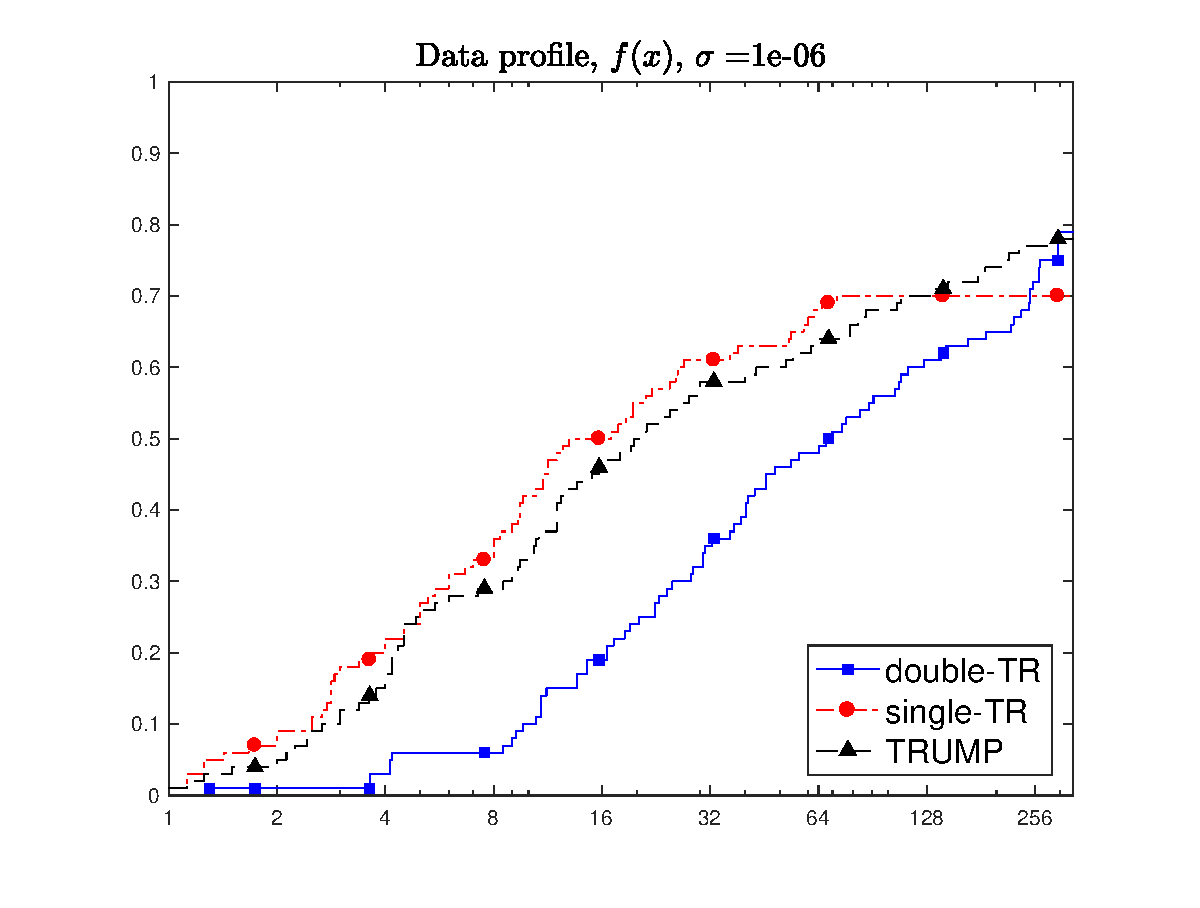
\includegraphics[width=.48\textwidth]{data_profile6f.eps} 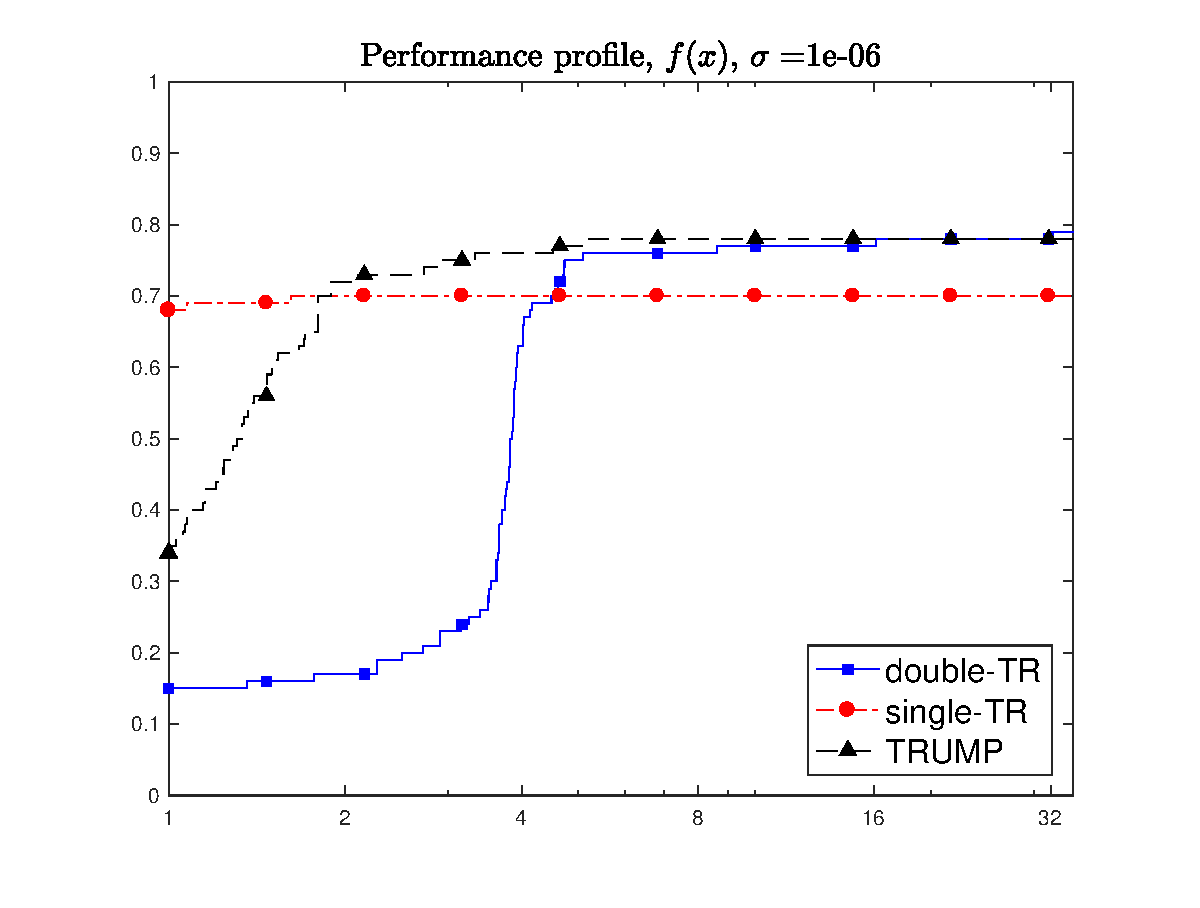
\includegraphics[width=.48\textwidth]{perf_profile6f.eps} 

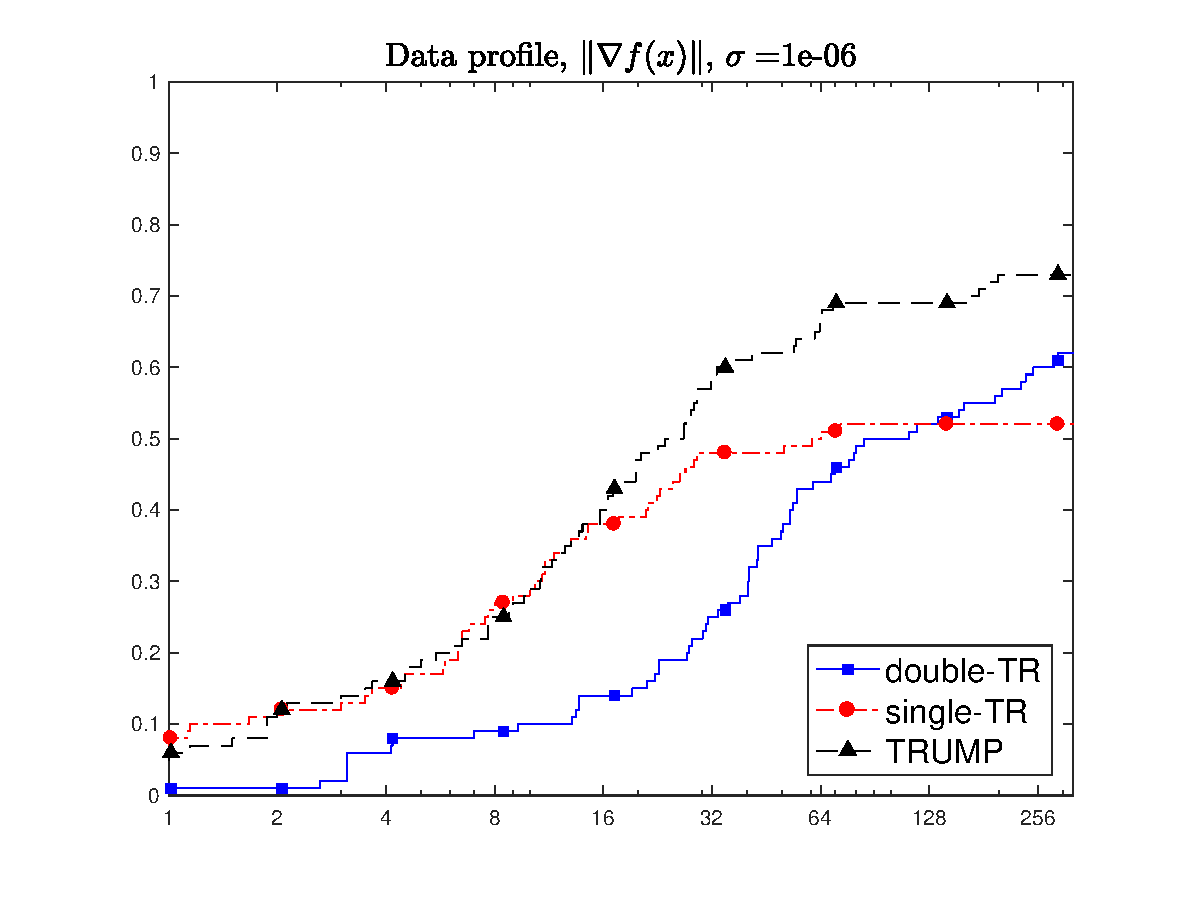
\includegraphics[width=.48\textwidth]{data_profile6g.eps} 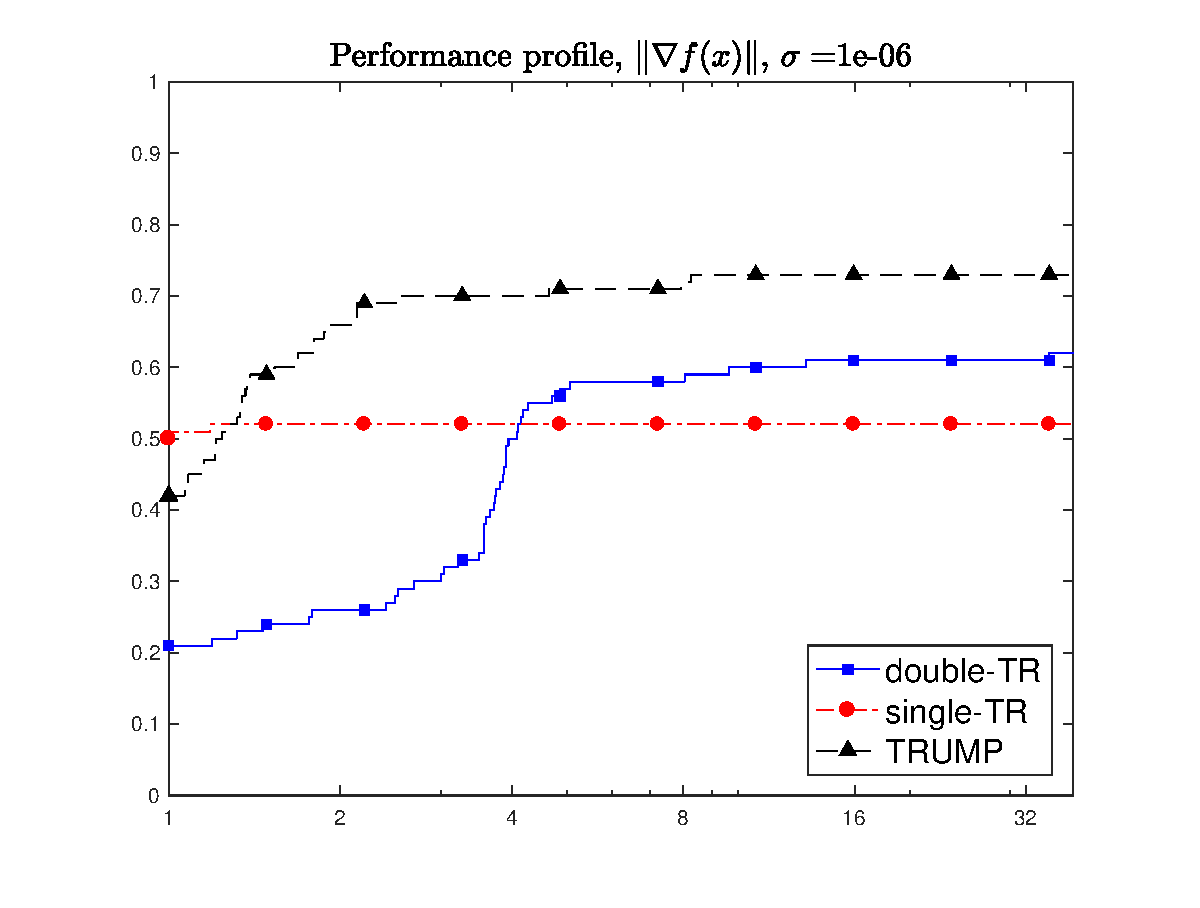
\includegraphics[width=.48\textwidth]{perf_profile6g.eps} 
\caption{Data profiles (left) and performance profiles (right) in terms of both the value of $f(x)$ (top) and gradient norm $\|\nabla f(x)\|$ (bottom). Threshold was chosen as $\sigma = 10^{-6}$.}
\end{figure}

\begin{figure}
\label{fig:cutest_profiles_mf2}
\includegraphics[width=.48\textwidth]{data_profile6f-mf2.eps} 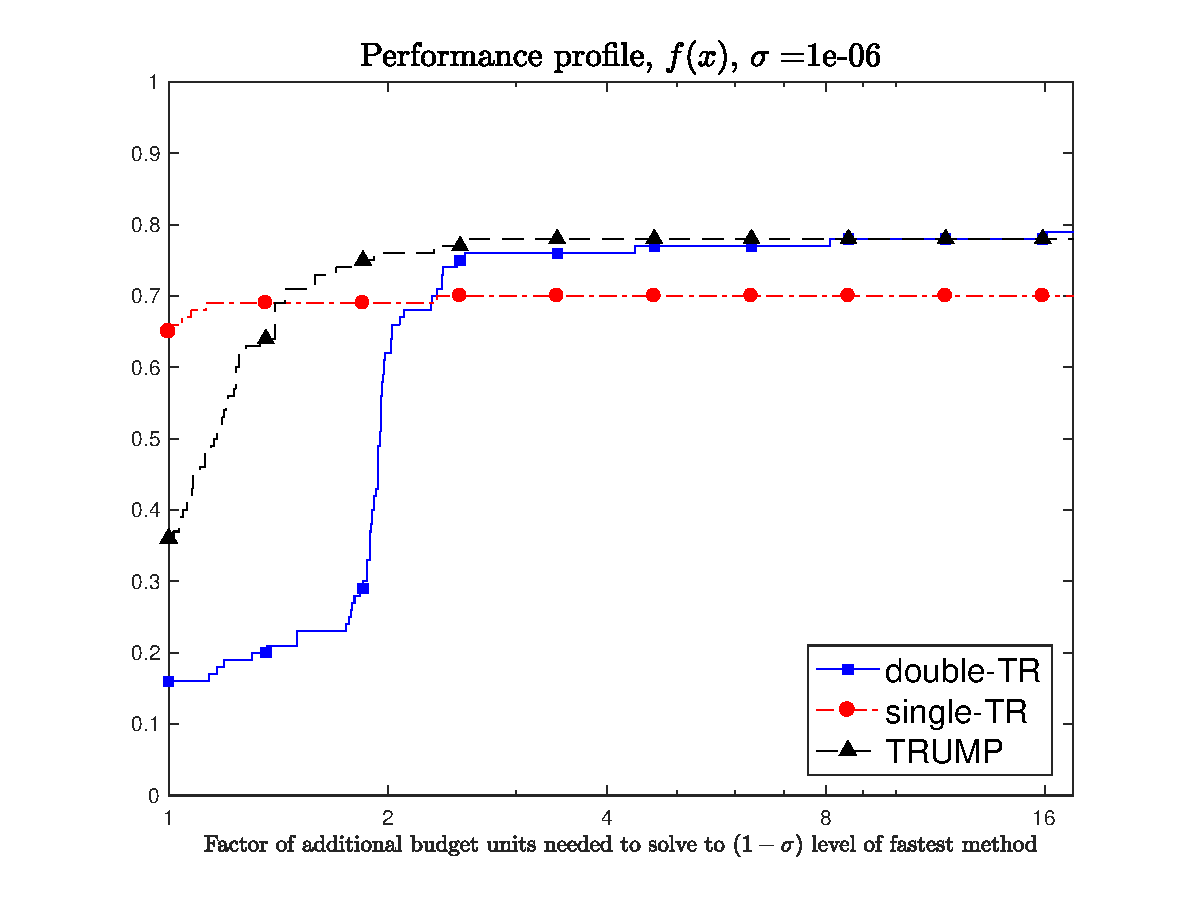
\includegraphics[width=.48\textwidth]{perf_profile6f-mf2.eps} 

\includegraphics[width=.48\textwidth]{data_profile6g-mf2.eps} 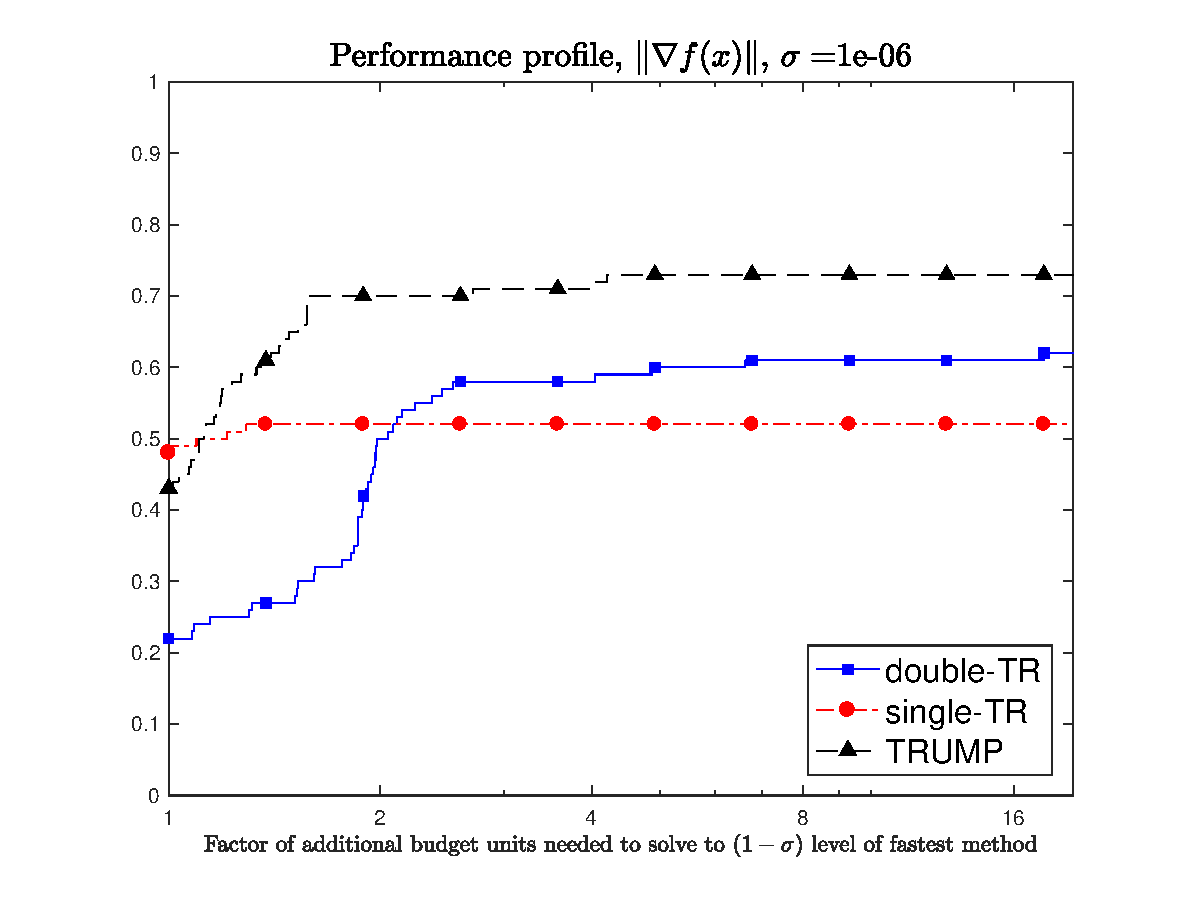
\includegraphics[width=.48\textwidth]{perf_profile6g-mf2.eps} 
\caption{Same as \figref{cutest_profiles}, but with the factor of relative costs between single and double set to 2, instead of 4.}
\end{figure}
\section{Conclusion, Future Work}
\label{sec:conclusion}
\bibliographystyle{unsrt}  
\bibliography{references}

\end{document}
